\documentclass{article}

%%% PREAMBLE %%%%%%%%%%%%%%%%%%%%%%%%%%%%%%%%%%%%%%%%%%%%%%%%%%%%%%%%%%%%%%%%%%%
% Title of the paper:
\newcommand{\hemaClassTitle}{\hemaClass{}: Online one-by-one normalization and classification of hematological malignacies}

% Load packages
\usepackage{fullpage} % Larger margins
\usepackage{amssymb,amsmath}
\usepackage{authblk}  % For author affiliations
\usepackage[hypertexnames=false]{hyperref} % For urls and hyperlinks
\usepackage{graphicx}
\usepackage[numbers,sort]{natbib}
\usepackage{cite} % Make references as [1-4], not [1,2,3,4]

% To do notes
\usepackage[
%  disable, %turn off todonotes
  colorinlistoftodos, %enable a coloured square in the list of todos
  textwidth=2cm, %set the width of the todonotes
  textsize=scriptsize, %size of the text in the todonotes
  ]{todonotes}

% Macros
\newcommand{\hemaClass}{\href{http://hemaClass.org}{\texttt{hemaClass.org}}}
\newcommand{\R}{\textsf{R}}
\newcommand{\pkg}[1]{\textbf{#1}}

\DeclareMathOperator*{\median}{median}
\DeclareMathOperator*{\std}{std}

% Hypenation
\hyphenation{Chemo-resistance}


%%%%%%%%%%%%%%%%%%%%%%%%%%%%%%%%%%%%%%%%%%%%%%%%%%%%%%%%%%%%%%%%%%%%%%%%%%%%%%%%

\title{\hemaClassTitle{}}

\author[1]{Steffen Falgreen\thanks{Shared first authorship}}
\author[12]{Anders Ellern Bilgrau$^\ast$}
\author[12]{Lasse Hjort Jakobsen}
\author[12]{Jonas Have}
\author[12]{Kasper Lindblad Nielsen}
\author[1]{Tarec Christoffer El-Galaly}
\author[1]{Julie St{\o}ve  B{\o}dker}
\author[1]{Alexander Schmitz}
\author[3]{Ken H. Young}
\author[12]{Hans Erik Johnsen}
\author[12]{Karen Dybk{\ae}r}
\author[12]{Martin B{\o}gsted\thanks{To whom correspondence should be addressed (\texttt{mboegsted@dcm.aau.dk})}}

\affil[1]{Department of Haematology, Aalborg University Hospital}
\affil[2]{Department of Clinical Medicine, Aalborg University}
\affil[3]{Department of Hematopathology, MD Anderson Cancer Center}

% Steffen Falgreen - sfl@rn.dk
% Anders Ellern Bilgrau - anders.ellern.bilgrau@gmail.com
% Lasse Hjort Jakobsen - lasse.j@rn.dk
% Jonas Have - jonas.have@rn.dk
% Kasper Lindblad Nielsen - k.lindblad@rn.dk
% Tarec Christoffer El-Galaly - tarec.galaly@gmail.com
% Julie S.\  B\o dker - j.boedker@rn.dk
% Alexander Schmitz - alex.schmitz@rn.dk
% Hans E.\ Johnsen - haej@rn.dk
% Karen Dybk\ae r - k.dybkaer@rn.dk
% Martin B\o gsted - martin.boegsted@rn.dk

\begin{document}

\maketitle
\phantomsection
\addcontentsline{toc}{section}{Abstract}
\begin{abstract}
\parttitle{Background} %if any
Dozens of genomics based cancer classification systems have been introduced with prognostic, diagnostic, and predictive capabilities.
However, they often employ complex algorithms and are only applicable on whole cohorts of patients, making them difficult to apply in a personalized clinical setting.
\\\parttitle{Results}
This prompted us to create \hemaClass{}, an online web application providing an easy interface to one-by-one microarray based risk classifications of diffuse large B-cell lymphoma (DLBCL) and multiple myeloma (MM) into cell-of-origin and chemotherapeutic sensitivity classes.
As laboratory specific effects cannot be accounted for in true one-by-one microarray normalization, \hemaClass{} optionally allows the user to supply a reference dataset to increase the accuracy of the classifications. Classification results for one-by-one array pre-processing with and without a user supplied reference dataset were compared to cohort based classifiers in $4$ publicly available datasets.
Overall, one-by-one and reference based normalization yield satisfactory inter-method agreements across all datasets.
The website is essentially the \R{}-package \pkg{hemaClass} accompanied by a Shiny web application.
The well-documented package can be used to run the website locally or to use the developed methods programatically.
\\\parttitle{Conclusions}
The website and \R{}-package is relevant for biological and clinical lymphoma researchers as it provides reliable and swift methods for calculation of disease subclasses.
The proposed one-by-one pre-processing methods are relevant for all researchers using microarrays.
\medskip\\
\textbf{Keywords:~}
Diffuse Large B-Cell Lymphoma; Multiple Myeloma; Classification; Chemosensitivity; Microarray; Pre-processing; Robust Multichip Average; Gene expression profiling; Cell of origin; Affymetrix Human Genome U133 Plus 2 microarrays
\end{abstract}



\section{Background}
In addition to current clinically used risk factor scoring systems several independent gene expression profile (GEP) based risk stratifications have been proposed with biological and clinical significance in hematological cancers.
Although drug targetable genes which are only expressed in subtypes of the e.g.\ DLBCL tumours have been identified, they are not readily applicable in clinical research and routine settings due to lack of available routine diagnostic tests \citep{Jaffe2009, Sehn2014}.

\citet{Alizadeh2000} developed an important example of a biological sub-classification of lymphoma.
On the basis of GEP analyses, DLBCL cases were assigned to categories of activated B-cell phenotype (ABC) or germinal center B-cell phenotype (GCB) with different clinical outcomes.
The validity of this classification and its prognostic importance have been confirmed in a number of later studies \citep{Rosenwald2002a,Hans2004,Poulsen2005,Lenz2008a,Monti2012a}.
Recently, we have refined the ABC/GCB subclassification of DLBCL to include a B-cell Associated Gene Signature (BAGS) classifier \citep{DybkaerBoegsted2015} capable of classifying DLBCL samples into $5$ different B-cell subtypes:
Naive (N), Centrocyte (CC), Centroblast (CB), Memory (M), and Plasmablasts (PB).
For example, the BAGS classifier stratifies the GCB subclass into a CC subtype with superior survival as compared to the CB subtype \citep{DybkaerBoegsted2015}, which opens up for considering different treatment regimes in the GCB class of patients.
In another study \citep{Falgreen2015} we developed classification based resistance gene signatures (REGS) for the most prominent drugs used in the treatment of DLBCL patients:
Cyclophosphamide (C), Doxorubicin (H), and Vincristine (O).
However, these and most existing algorithms are only applicable in the presence of whole cohorts of patients making them difficult to apply in a routine clinical setting.

The traditional lymphoma staging and risk classification systems are based on the Ann Arbor classification for staging of lymphoma (extent of disease and extranodal involvement) and simple prognostic tools such as the international prognostic index (IPI, \citep{IPI}) for large cell lymphoma and the Follicular Lymphoma International Prognostic Index (FLIPI, \citep{FLIPI}), both derived from patient age, performance status, easy available blood tests, and disease stage.
Due to the simplicity of these clinical risk stratification algorithms they are still the most widely used risk scoring systems today.
Risk stratification according to these algorithms has been systematized and made easily accessible for desktop, online, and even smart-phone use.
However, easily accessible molecular classification methods are lacking behind and thereby delaying the translation of new molecular findings into clinical practice.
A few methods exist for cancer types other than lymphoma, including acute myeloid leukemia (AML) \citep{Huang2009}.
To the best of our knowledge, quite surprisingly, no tools have been developed for use in the lymphoma field despite very early promising results in the molecular biomarker field.
An accessible Windows based application has been published for ABC/GCB classification \citep{Care2013}.
Although \citet{Care2013} develop a new ABC/GCB classifier which is stable across microarray technologies and trial centres, the ABC/GCB classifier is potentially biased towards classes which differentiate the prognosis and not biology.
This bias arises as the ensemble of classifiers are chosen on basis of their ability to separate survival.

In clinical settings, the methods need to be applicable for a single patient sample and straightforward to use.
This prompted us to develop an easy accessible and flexible web-based tool for ABC/GCB, BAGS, and REGS classification which is capable of computing our recently developed classifiers for microarray data based on the Affymetrix's Human Genome U-133 Plus 2 arrays.
The classifications made by the web-based tool \hemaClass{} are compared to the existing state-of-the-art and approved ABC/GCB classifications of DLBCL.
We believe that \hemaClass{} will provide a novel and user-friendly concept for bringing complex molecular classification of diseases more swiftly into daily clinical practice.
As already delineated, this paper primarily describes developed classification schemes for DLBCL although MM classification is currently also featured on the website.
A more extensive treatment of MM classification schemes is in preparation and will be implemented on \hemaClass{}.


\section{Implementation}

\subsection{Classification workflow}
The analysis workflow of \hemaClass{} can be divided into four parts:
(1) Three reference datasets which have been pre-processed and prepared offline are loaded upon server start,
(2) a graphical user interface with upload and input facilities,
(3) a server handling the online processing and classification of the user input, and
(4) the resulting classifications available for download and inspection via the user interface.
The workflow architecture is illustrated in Figure \ref{fig:webtooldiagram}.

\begin{figure}
\begin{center}
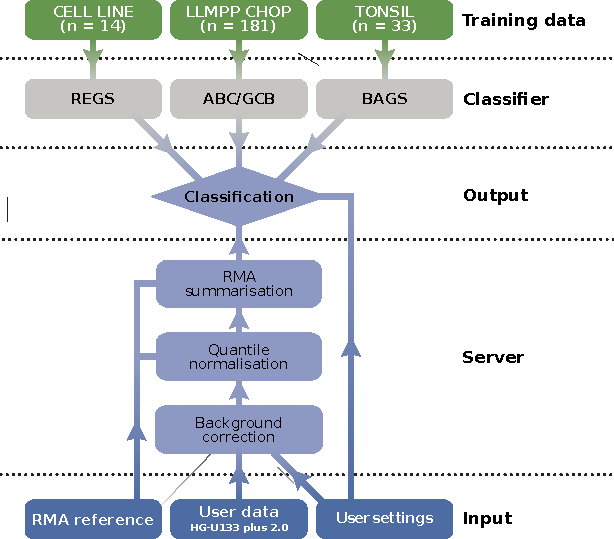
\includegraphics[width=0.5\textwidth]{figures/figure1.pdf}
\end{center}
\caption{Diagram of the workflow architecture.}
\label{fig:webtooldiagram}
\end{figure}


\subsection{Software availability and technical details}
The interactive web application available at \url{hemaclass.org} was created using the statistical programming language \R{} \citep{RCoreTeam}, the software package \pkg{shiny} \citep{shiny}, and the accompanying Linux server software.
All \hemaClass{} functionality, including the RMA normalization and classification procedures, are available through the accompanying package \pkg{hemaClass} based on a number of packages from the Comprehensive R Archive Network \citep{RCoreTeam} and the Bioconductor environment \citep{Gentleman2004}.
The Shiny server handles the interaction between the front end web application and the back end \R{} processing.
The back end is essentially the well-documented \pkg{hemaClass} package which can be utilized as a programmatical interface to the functionality of the website.
However, the package also allows users to run a local instance of the website if one wishes to avoid uploading large files to our server.
The development and latest version of \pkg{hemaClass} is open source and freely available at \url{https://github.com/oncoclass/hemaclass} for sharing, modification, and redistribution.
All bug-reports, suggestions, and comments on the website or package are welcome following the latter link.
The regular RMA pre-processing is carried out with the Bioconductor package \pkg{affy} \citep{Gautier2004}.
Core functions for the one-by-one and reference based RMA pre-processing are written in \textsf{C++} and imported to \R{} using \pkg{Rcpp} and \pkg{RcppArmadillo} \citep{Rcpp2013,Eddelbuettel2011,RcppArmadillo,Sanderson2010}.





\subsection{Data overview}
The seven gene expression datasets used in this paper are summarized in Table \ref{table:01}.
All GEP data are on the Affymetrix GeneChip HG-U133 Plus 2.0 array and available at the Gene Expression Omnibus (GEO) \citep{Barrett2013} website (\url{http://www.ncbi.nlm.nih.gov/geo/}).
To establish the classifiers the following datasets are used:
\begin{enumerate}
  \item Gene expressions from $181$ CHOP treated DLBCL patients are used to establish the ABC/GCB classifier.
  This cohort will be referred to as the \emph{LLMPP CHOP} (Lymphoma/Leukemia Molecular Profiling Project CHOP) cohort \citep{Lenz2008a}.
  The cohort is also used as a default reference set throughout the paper for normalization of arrays.
  \item The BAGS classifier is based on gene expression data from eight human tonsils sorted in five B-cell subsets.
  This dataset will be referred to as the \emph{Tonsil dataset} and it is also used for scaling of gene expression data for BAGS classification \citep{DybkaerBoegsted2015}.
  \item The REGS classifiers are based on a panel of $12$ Multiple Myeloma (MM) and $14$ DLBCL cell lines.
  This panel will be referred to as \emph{BCELL26}.
  The DLBCL part of the cell line panel is used for scaling of patient data and this part of the dataset will be referred to as   \emph{DLBCL14} \citep{Falgreen2015}.
\end{enumerate}
For validation the following four DLBCL cohorts are used:
\begin{enumerate}
  \item[4.] The Aalborg OCT cohort (\emph{CHEPRETRO}) of $89$ Danish DLBCL patients undergoing first-line treatment at Aalborg University Hospital \citep{DybkaerBoegsted2015}.
  The clinical dataset is as registered in the National Clinical Quality Database for Malignant Lymphoma (LYFO, \url{lymphoma.dk}) \citep{Gang2012}.
  \item[5.] The International DLBCL Rituximab-CHOP Consortium MD Anderson (\emph{IDRC}) cohort of $470$ DLBCL patients treated with R-CHOP first-line therapy \citep{Visco2012}.
  Note, that these samples are formalin-fixed, paraffin-embedded (FFPE).
  \item[6.] The Lymphoma/Leukemia Molecular Profiling Project R-CHOP (\emph{LLMPP R-CHOP}) cohort of $233$ DLBCL patients treated with R-CHOP first-line therapy \citep{Lenz2008a}.
  \item[7.] The Mayo-Dana-Farber Cancer Institute (\emph{MDFCI}) cohort of $90$ DLBCL patients treated with R-CHOP first-line therapy \citep{Monti2012a}.
\end{enumerate}
The GEO datasets were downloaded using the \R{}-package \pkg{DLBCLdata} \citep{DLBCLdata}.

\begin{table}%[htb]
\small
\caption{Overview of used datasets and GEO accession numbers.}
\label{table:01}%
\begin{center}
\begin{tabular}{rlclll}
\hline\hline
No. & Dataset & $n$ & Usage & GEO number & Ref.
\\
\hline
1. & LLMPP CHOP & 181 & Training & GSE10846 & \cite{Lenz2008a}
\\
2. & Tonsil & 33 & Training & GSE56315 & \cite{DybkaerBoegsted2015}
\\
3. & BCELL26 & 26 & Training & GSE53798 & \cite{Falgreen2015}
\\
4. & CHEPRETRO & 89 & Validation & GSE56315 & \cite{DybkaerBoegsted2015}
\\
5. & IDRC & 470 & Validation & GSE31312 & \cite{Visco2012}
\\
6. & LLMPP R-CHOP & 233 & Validation & GSE10846 & \cite{Lenz2008a}
\\
7. & MDFCI & 90 & Validation & GSE34171 & \cite{Monti2012a}\\
\hline
\end{tabular}
\end{center}
\end{table}




\subsection{One-by-one RMA normalization}
Recall that robust multichip average (RMA) pre-processing consists of three steps in the order:
(1) Background correction,
(2) quantile normalization, and
(3) summarization of probes to probe-sets \citep{Irizarry2003,Irizarry2003b}.
Confer \citet{Bolstad2004} for a comprehensive account on RMA.
Both the quantile normalization and summarization procedures of RMA are cohort based and hence need to be altered to facilitate a one-by-one RMA pre-processing scheme.
As quantile normalizer, the empirical cumulative distribution function (ECDF) of the mean of the sample quantiles of the RMA background corrected LLMPP CHOP reference data is used in place of the usually applied ECDF of the mean of the sample quantiles of the user supplied data \citep{Bolstad2003}.
To mimic the summarization procedure of RMA \citep{Irizarry2003b} the probe effects estimated by median polish for the LLMPP CHOP reference data is subtracted all probes of the user data.
The RMA pre-processed expression value for each probe-set is then estimated as the median of the associated probes.
Finally, before classification the median of each probe-set in the LLMPP CHOP is subtracted from the corresponding probe-set in the user data.
This ensures identical classification probabilities whether data is supplied as a cohort or one-by-one.

To accommodate laboratory and sample preparation specific effects different from the LLMPP CHOP reference data, \hemaClass{} allows the user to upload an alternative dataset which is to be used in place of LLMPP CHOP as reference.
In this paper the reference datasets consisted of $30$ randomly selected samples from a given study.
The three pre-processing methods will be referred to as \emph{cohort}, \emph{one-by-one}, and \emph{reference based} normalization.


\subsection{Classification methods}

\subsubsection{Elastic nets}
Logistic and multinomial regression are used in all classification methods available at \hemaClass{}.
However, in GEP experiments, the number of probe-sets present on the microarray always outnumbers the sample size.
Collinearity present among the features further aggravates the problem of identifying genes responsible for the underlying biological mechanism.
Regression under these ill-posed circumstances is typically handled by so-called regularization.
Here the elastic net penalty \citep{Friedman2010, Zou2005} is used which is a combination of the lasso \citep{Tibshirani1996} and ridge regression \citep{Hoerl1970}.
Similar to the lasso, this penalty ensures simultaneous variable selection and model estimation by forcing small coefficients to be zero, yielding sparse solutions.
In contrast to the lasso, the elastic net penalty is capable of selecting more variables than samples.

The elastic net penalty contains two parameters $\alpha$ and $\lambda$.
The parameter $\alpha$ interpolates the elastic net penalty between the ridge and the lasso penalty which corresponds to values of $0$ and $1$, respectively.
The parameter $\lambda$ determines the amount of shrinkage of the coefficients with larger values inducing more shrinkage until no variables are contained in the model.
Regularized logistic and multinomial regression are performed with the \R{}-package \pkg{glmnet} \citep{Friedman2010}.

\subsubsection{ABC/GCB classification}
The ABC/GCB classifier is established using logistic regression with an elastic net penalty on the LLMPP CHOP cohort.
Of the $181$ patients $74$ were ABC, $76$ were GCB, and $31$ were non-classified.
Using the $150$ patients classified as either ABC or GCB the dichotomous classifier capable of assigning each sample an estimate of the probability of being ABC was established.

To avoid over-fitting and limit the number of noise contributing genes, the elastic net parameters $\alpha$ and $\lambda$ were chosen through $10$ fold cross-validation.
The parameter $\alpha$ was varied between $0.1$ and $1$ with step size $0.025$ and $\log(\lambda)$ was varied between $-10$ and $2$ with step size $0.06$.
The optimal combination of the parameters and thereby the number of probe-sets were found at the values minimising the deviance.
The results of the cross validations are shown in Supplementary Figure \ref{fig:crossval}.
The minimum $0.13$ was attained at $\alpha = 0.15$ and $\log(\lambda) = -7.41$ resulting in a gene expression classifier consisting of $381$ probe-sets.

When a tumour sample is classified according to the ABC/GCB classifier using one-by-one normalization the data is used directly when classifying. However, when a tumour sample is classified according to the ABC/GCB classifier using reference based normalization the associated gene expressions are rescaled probe-set wise by the standard deviation of the LLMPP CHOP data divided by the standard deviation of the user supplied reference data.

\subsubsection{REGS classification}
\label{sec:regsmethods}
In the paper by \citet{Falgreen2015} REGS classifiers were established for prediction of resistance to the drugs C, H, and O.
The classifiers were established on BCELL26 using regularized logistic regression analogous to the procedure described for the aforementioned ABC/GCB classifier.

The probability of resistance to the combination therapy $p_{CHO}$ is estimated based on the probabilities of drug resistance toward each of the three drugs $P_C$, $P_H$, and $P_O$, respectively.
This probability is calculated by a formula derived as the posterior probability of being resistance given resistance towards each of the individual drugs under the assumption of conditional independence and uniform priors.
The formula is also known as Graham's formula,
\begin{equation*}
  P_{CHO} = \frac{P_C P_H P_O}{P_C P_H P_O + (1 - P_C)(1 - P_H)(1 - P_O)},
\end{equation*}
and derived in Supplementary Section \ref{sec:graham}.
If a drug is left out in the combination therapy the drug is simply removed from the formula.
This appoach to resistance to the combination therapy was used in \citet{Falgreen2015}.

When a tumour sample is classified according to the REGS classifiers the associated gene expressions are rescaled probe-set wise by the standard deviation of DLBCL14 divided by the standard deviation of the LLMPP CHOP dataset.
Similarly to the other classifiers the LLMPP CHOP cohort is replaced by the user reference dataset, if supplied.

Resistance classifiers for other chemotherapeutic drugs and diseases are also available on \hemaClass{} though established elsewhere \citep{Boegsted2011,Bogsted2013,Laursen2014}.
The Rituximab sensitivity classifier of \citet{Laursen2014} and \citet{Laursen2015} is based upon an elastic net approach, like above, however using three classes.
The Melphalan sensitivity classifier of \citet{Boegsted2011} uses sparse partial least squares to assign the classes sensitive, intermediate, and resistant to samples.
This classifier was developed for multiple myeloma (MM) patients and thus based on other data \citep{Boegsted2011}.
A classifier for dexamethasone is still considered experimental and currently available only in the package.


\subsubsection{BAGS classification}
The BAGS classifier established by \citet{DybkaerBoegsted2015} was based on multinomial regression regularized by an elastic net penalty.
The classifier was trained on the Tonsil dataset in a manner similar to the ABC/GCB classifier.

When a tumour sample is classified according to the BAGS classifier the associated gene expressions are rescaled probe-set wise by the standard deviation of the Tonsil data divided by the standard deviation of the LLMPP CHOP dataset.
If the user supplies a reference dataset this is used in place of LLMPP CHOP.
The rescaling is performed to make the data comparable to the Tonsil dataset.


\subsection{Inter-method reproducibility assessments}
To evaluate the reproducibility of the class probabilities obtained through cohort based normalization and one-by-one as well as reference based normalization, Pearson's correlation coefficient for the logit-transformed probabilities and $95\%$ confidence interval (CI) were calculated for each classifier and dataset.
The identity and \emph{total} least square regression lines were compared to assess bias in the estimated probabilities \citep{CHEN1989}.
Total least squares regression was used as errors are present in both classification probabilities.

For each classifier the associated categories were obtained by thresholding the estimated probabilities.
The ABC/GCB classifier was thresholded by $0.1$ and $0.9$, i.e.\ a tumour sample was classified as ABC when the estimated probability exceeds $0.9$, GCB when it is beneath $0.1$, and unclassified otherwise.
For the BAGS classifier a tumour was classified as the class N, CB, CC, M, or PB with the highest probablity, if the associated probability exceeded $0.5$ and unclassified when this threshold was not met for any subtype.
For the REGS classifiers, C, H, O, and CHO combined, the threshold used were the $33\%$ and $66\%$ percentile of the estimated probabilities.
The classifiers were applied to datasets using the cohort, one-by-one, and reference based RMA normalization.
After thresholding the class probabilities confusion matrices were created.
From these the rate of agreement (or accuracy), Cohen's weighted $\kappa$, and corresponding $95\%$ CIs were computed to assess the agreement between the determined classes.


\section{Results}
\subsection{Using \hemaClass{}}
The website is an easy-to-use, interactive interface for the \pkg{hemaClass} package with the desired RMA normalization and the classification methods selected by the user.
The usage of the website is largely self-explanatory with context-dependent boxes aiding users with further information, warnings, or errors.
A comprehensive tutorial and guide to both the website and package is provided on the website or by running \texttt{vignette("howto")} in \R{}.
Users upload patient samples which are normalized and classified depending on settings chosen by the users.
A text summary of the results and a plot of the predicted progression free survival and overall survival is optionally provided for each patient sample.
These predictions are based on the patient survival data from LLMPP - RCHOP , MDFCI, and IDRC, as combined in \citet{DybkaerBoegsted2015}, using a Cox proportional hazard's regression with predictors IPI, at levels $0,1,2,4,5$, and a factor combining the ABC/GCB and BAGS classes, at levels ABC, GCB, GCB-CC, GCB-CB, and NC.



\subsection{ABC/GCB classification}
In order to classify patients as ABC/GCB based on the implemented one-by-one normalization method a classifier based on the regularised logistic regression was established.
The classifications were evaluated in the four clinical cohorts CHEPRETRO, MDFCI, IDRC, and LLMPP R-CHOP, which have all been classified according to the Wright's naive Bayes classifier \citep{Wright2003,Lenz2008a}.
The rate of agreement between the two classifiers are shown in Table \ref{tab:ABCGCBclassifier}.
Note that unclassified samples were included in the estimation of this rate i.e.\ a patient classified as ABC by one classifier but unclassified by the other is considered an error.
The table also includes the alternative measure of agreement, Cohen's weighted $\kappa$, were misclassifications involving the unclassified group are weighted by $1/2$.
The accompanying confusion matrices are shown in the first rows of Supplementary Table \ref{tab:confusionABCGCBHEMA}.

The logit probability of being ABC estimated using the established cohort-based classifier was compared to the corresponding estimate obtained through the one-by-one based classification scheme in Figure \ref{fig:ABCGCBDrug}A for CHEPRETRO.
The probabilities estimated through the two methods are very similar.
However, the probabilities estimated under one-by-one normalization are slightly uncalibrated (or biased) and skewed upwards, indicating that different cut points might be used for the classifications.
By normalizing to a reference set of $30$ randomly selected samples from CHEPRETRO this error and bias is greatly minimised as shown in Figure \ref{fig:ABCGCBDrug}B.

For both methods, patients are classified as ABC when the estimated probability exceeds $0.9$ and GCB when it is below $0.1$.
In Table \ref{tab:classALL} the resulting classifications are compared in terms of accuracy and Cohen's weighted $\kappa$ for one-by-one normalization and four validation datasets normalized to 30 internally sampled reference samples.
CHEPRETRO, MDFCI, IDRC, and LLMPP R-CHOP all show a high Cohen's weighted $\kappa$ and good rate of agreement, considering that misclassifications involving unclassified samples count as errors.
The reduced rate of agreement and Cohen's weighted $\kappa$ using one-by-one pre-processing in IDRC may be due to the samples being FFPE although this seems to be remedied by reference based pre-processing.
The accompanying confusion matrices are shown in the lower part of Supplementary Table \ref{tab:confusionABCGCBHEMA}.
Note, changes in predicted classes are mainly due to shifts into NC from ABC or GCB.
Direct disagreements between the classifiers are seemingly rare and only occurs in the IDRC dataset.

%latex.default(table2, file = "tables/table2.tex", title = "Dataset",     caption = caption, label = "tab:ABCGCBclassifier", size = "small")%
\begin{table}[!tbp]
{\small
\caption{Comparison of ABC/GCB classification performed using Wright's naive
Bayes classifier \citep{Wright2003} and the established elastic net classifier
both based on cohort normalization.
The second column shows the accuracy of the
classifiers with $95\%$ CI. The third column shows the Cohen's weighted
$\kappa$ with $95\%$ CI.\label{tab:ABCGCBclassifier}} 
\begin{center}
\begin{tabular}{lll}
\hline\hline
\multicolumn{1}{l}{Dataset}&\multicolumn{1}{c}{Accuracy}&\multicolumn{1}{c}{Cohen's $\kappa$}\tabularnewline
\hline
CHEPRETRO&$0.94~(0.87, 0.98)$&$0.94~(0.88, 1.00)$\tabularnewline
MDFCI&$0.78~(0.68, 0.86)$&$0.77~(0.66, 0.88)$\tabularnewline
IDRC&$0.82~(0.79, 0.86)$&$0.80~(0.76, 0.85)$\tabularnewline
LLMPP R-CHOP&$0.91~(0.86, 0.94)$&$0.90~(0.85, 0.96)$\tabularnewline
\hline
\end{tabular}\end{center}}

\end{table}


\begin{figure}
\begin{center}
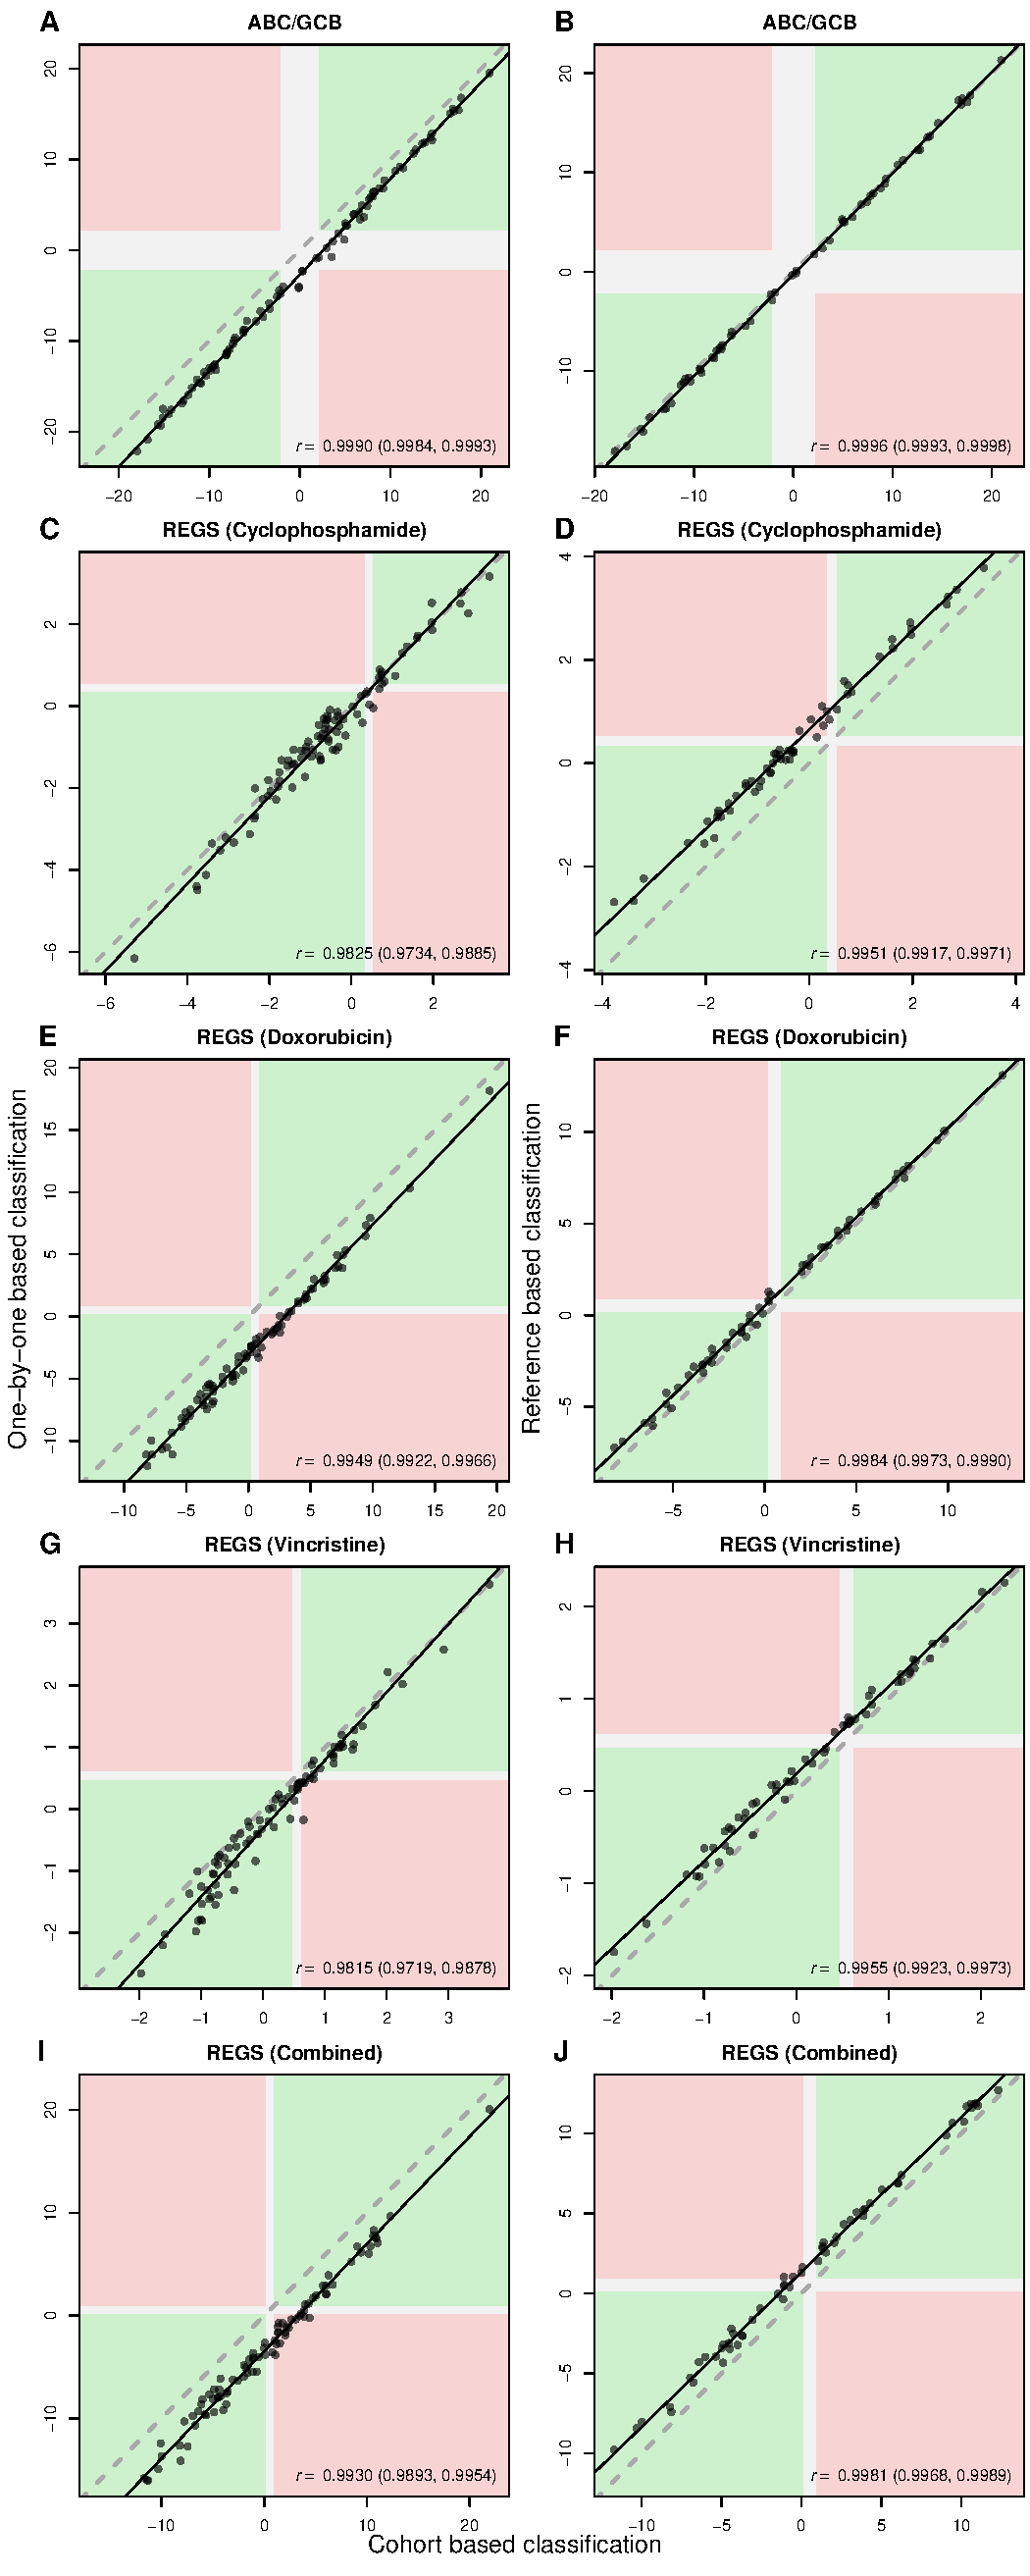
\includegraphics[width=0.375\textwidth]{figures/figure2.pdf}
\end{center}
\caption{
Comparison of logit probabilities for the ABC/GCB and REGS classifiers obtained through one-by-one and reference based normalization against cohort normalization.
The areas marked with green indicate patients with similar classification between cohort based normalization and one-by-one normalization (A, C, E, G, I)  and reference based RMA normalization (B, D, F, H, J) .
Contrary, the areas marked with red indicate complete misclassifications.
For ABC/GCB and REGS the white areas indicate unclassified and intermediate sensitivity, respectively, in at least one of the classifiers.
The dashed and solid line show the identity and total least squares line, respectively.
}
\label{fig:ABCGCBDrug}
\end{figure}

\begin{figure}
\begin{center}
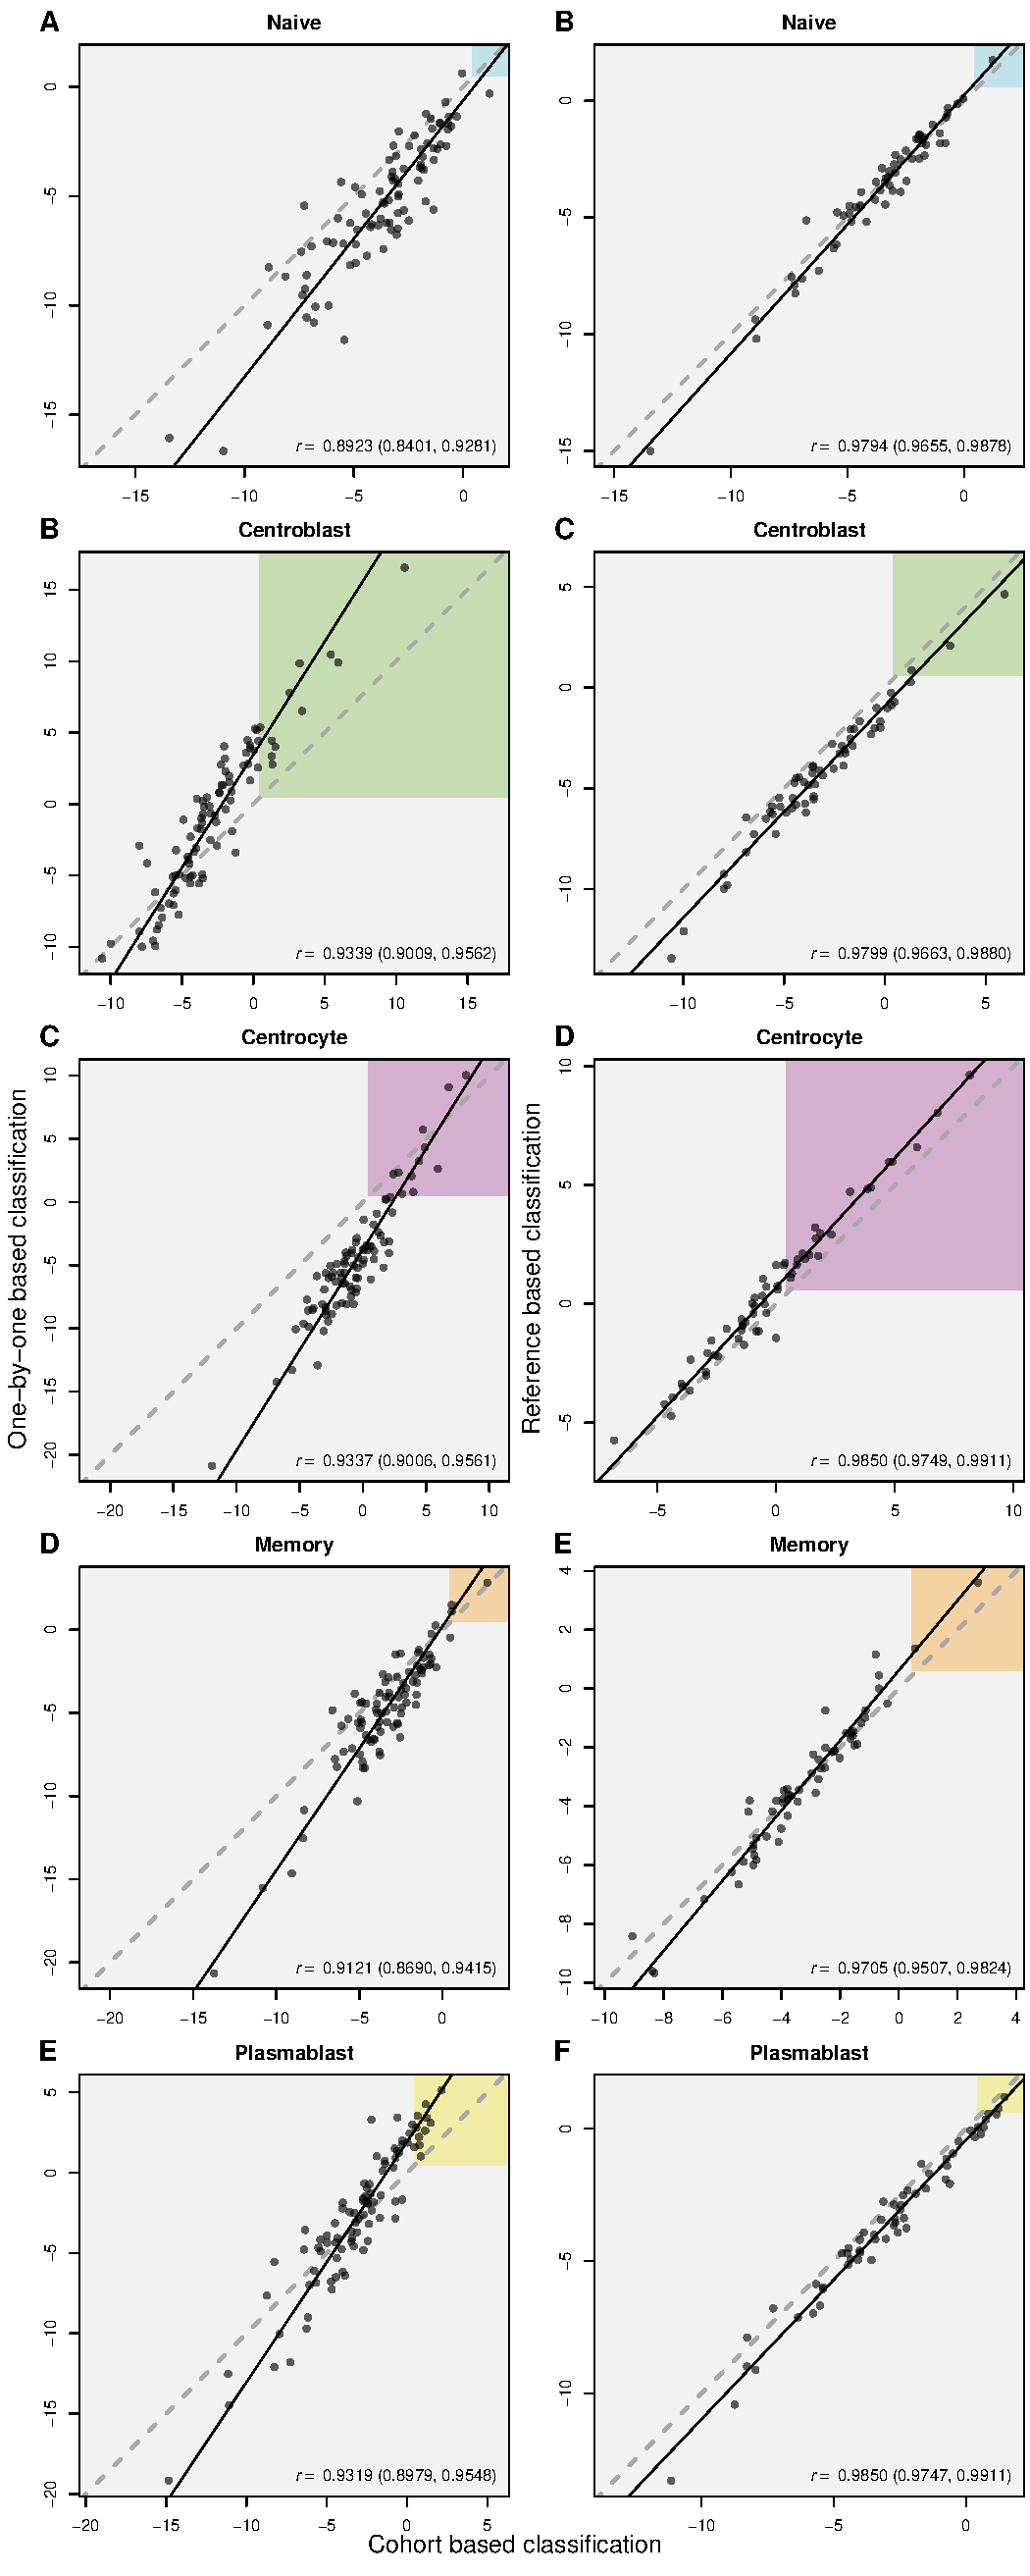
\includegraphics[width=0.375\textwidth]{figures/figure3.pdf}
\end{center}
\caption{
Comparison of logit probabilities for the BAGS classifier obtained through one-by-one and reference based normalization against cohort normalization.
The coloured regions in the figure correspond to a threshold probability of $0.5$.
The dashed and solid line show the identity and total least squares line, respectively.
}
\label{fig:Bagscorr}
\end{figure}
\newpage



\subsection{REGS classification}
The probability of sensitivity towards each of the three drugs C, H, and O was estimated using \hemaClass{} both in terms of one-by-one and reference based normalization.
The logit probabilities of sensitivity are plotted against those obtained by cohort based normalization in Figure \ref{fig:ABCGCBDrug} for CHEPRETRO data.
Panels C, E, G, and I show the plots based on one-by-one normalization and panels D, F, H, and J show the plots for the reference based normalization.
The probabilities obtained by one-by-one and cohort based normalization are comparable. However, similar to the other classifiers the one-by-one normalization leads to slightly skewed and biased probabilities, indicating that different cut points should be considered.
The probabilities obtained by the reference based normalization resembles the cohort based to a great extent indicating that similar well-calibrated probabilities are obtainable for different laboratories by supplying a reference set.

Based on the estimated probabilities, the patients were categorised as sensitive, intermediate, or resistant based on the thresholds specified in Section \ref{sec:regsmethods}.
The classes obtained by \hemaClass{} are compared to those obtained by the cohort based approach in Table \ref{tab:classALL} in terms of rate of agreement and Cohen's weighted $\kappa$.
The associated confusion matrices for one-by-one normalization and reference based normalization are shown in
Supplementary Table \ref{tab:confusiondrugonebyone} and
Supplementary Table \ref{tab:confusiondrugreference}, respectively.
Again, the reference based approach yields superior agreement with classifications using cohort based normalization.


\subsection{BAGS classification}
The BAGS classifier was evaluated in a manner similar to the ABC/GCB classifier.
The logit probability of a patient's tumour originating from one of the five subpopulations is again estimated by means of cohort, one-by-one, and reference based normalization.
The logit probabilities estimated by the one-by-one normalization is plotted against that of the cohort based normalization in Figure \ref{fig:Bagscorr} panels A, C, E, G, and I for CHEPRETRO.
The correlations between the logit probabilities are highly significant, although slightly skewed and biased.
To accommodate for this, the data was also normalized using a reference dataset.
The logit probabilities estimated by the reference based normalization is plotted against that estimated for the cohort based normalization in Figure \ref{fig:Bagscorr} panels B, D, F, H, and J for CHEPRETRO.
The reference based normalization removes much of the aforementioned bias.

Based on the probabilities estimated by means of each of the three normalization methods the patients of the four clinical cohorts are grouped into the BAGS.
The rate of agreement between the cohort based and one-by-one as well as reference based classifications is shown in Table \ref{tab:classALL} along with the Cohen's weighted $\kappa$.
The associated confusion matrices are shown in Supplementary Table \ref{tab:BAGShemaclass}.

%latex.default(table3, file = "tables/table3.tex", title = "",     rgroup = gsub("ABCGCB", "ABC/GCB", names(results)), cgroup = c("One-by-one pre-processing",         "Reference based pre-processing"), size = "scriptsize",     label = "tab:classALL", caption = caption)%
\begin{table}[!tbp]
{\scriptsize
\caption{Comparison of classifications obtained using cohort based
normalisation and \hemaClass{}.
The classifications are compared in terms of accuracy, Cohen's weighted
$\kappa$, and Pearson's correlation coefficient $r$ all supplied with $95\%$
CIs. The comparisons in the first and last three columns are based on the
one-by-one normalisation method and the reference based normalisation method,
respectively.\label{tab:classALL}} 
\begin{center}
\begin{tabular}{llllclll}
\hline\hline
\multicolumn{1}{l}{\bfseries }&\multicolumn{3}{c}{\bfseries One-by-one pre-processing}&\multicolumn{1}{c}{\bfseries }&\multicolumn{3}{c}{\bfseries Reference based pre-processing}\tabularnewline
\cline{2-4} \cline{6-8}
\multicolumn{1}{l}{}&\multicolumn{1}{c}{Agreement}&\multicolumn{1}{c}{Cohen's $\kappa$}&\multicolumn{1}{c}{Pearson's $r$}&\multicolumn{1}{c}{}&\multicolumn{1}{c}{Agreement}&\multicolumn{1}{c}{Cohen's $\kappa$}&\multicolumn{1}{c}{Pearson's $r$}\tabularnewline
\hline
{\bfseries ABC/GCB}&&&&&&&\tabularnewline
~~CHEPRETRO&$.88~(.79, .94)$&$.87~(.78, .97)$&$.999~(.998, .999)$&&$.98~(.91, 1.0)$&$.98~(.93, 1.0)$&$1.00~(.999, 1.00)$\tabularnewline
~~MDFCI&$.69~(.59, .78)$&$.68~(.53, .82)$&$.999~(.998, .999)$&&$.98~(.91, 1.0)$&$.98~(.85, 1.0)$&$1.00~(.999, 1.00)$\tabularnewline
~~IDRC&$.65~(.61, .69)$&$.62~(.57, .68)$&$.986~(.983, .988)$&&$.94~(.91, .96)$&$.93~(.90, .97)$&$.995~(.994, .996)$\tabularnewline
~~LLMPP R-CHOP&$.82~(.77, .87)$&$.82~(.74, .89)$&$.999~(.999, .999)$&&$.94~(.90, .97)$&$.94~(.90, .98)$&$.992~(.989, .994)$\tabularnewline
\hline
{\bfseries BAGS}&&&&&&&\tabularnewline
~~CHEPRETRO&$.57~(.46, .68)$&$.54~(.27, .82)$&-&&$.78~(.65, .88)$&$.74~(.34, 1.0)$&-\tabularnewline
~~MDFCI&$.54~(.43, .64)$&$.48~(.17, .79)$&-&&$.79~(.66, .88)$&$.81~(.30, 1.0)$&-\tabularnewline
~~IDRC&$.52~(.48, .57)$&$.42~(.32, .51)$&-&&$.79~(.75, .83)$&$.80~(.62, .97)$&-\tabularnewline
~~LLMPP R-CHOP&$.57~(.50, .63)$&$.54~(.37, .71)$&-&&$.82~(.76, .87)$&$.83~(.54, 1.0)$&-\tabularnewline
\hline
{\bfseries REGS}&&&&&&&\tabularnewline
~~CHEPRETRO&$.74~(.69, .78)$&$.71~(.65, .78)$&$.935~(.920, .947)$&&$.83~(.78, .88)$&$.82~(.76, .89)$&$.992~(.990, .994)$\tabularnewline
~~MDFCI&$.60~(.55, .65)$&$.55~(.48, .62)$&$.825~(.789, .855)$&&$.90~(.86, .94)$&$.89~(.83, .96)$&$.997~(.996, .997)$\tabularnewline
~~IDRC&$.52~(.49, .54)$&$.33~(.30, .36)$&$.661~(.636, .686)$&&$.84~(.82, .85)$&$.82~(.79, .84)$&$.984~(.983, .986)$\tabularnewline
~~LLMPP R-CHOP&$.58~(.55, .61)$&$.50~(.46, .54)$&$.811~(.788, .832)$&&$.89~(.87, .91)$&$.89~(.85, .92)$&$.992~(.991, .993)$\tabularnewline
\hline
\end{tabular}\end{center}}

\end{table}



\section{Discussion}
Despite the enormous resources spent on developing molecular based cancer classification systems,
most of these are still not available in daily clinical practice.
% there seems to be an inertial resistance to develop clinical applications.
To allow for fast validation of our recent findings \citep{DybkaerBoegsted2015, Falgreen2015}, we have developed an easily accessible web application that permits other users to apply ABC/GCB, BAGS as well as drug resistance classification on their own datasets.

The one-by-one and referece based classifications performed by \hemaClass{} were compared to those obtained using cohort based normalization in four clinical cohorts.
Even though gene expression data for the four cohorts were obtained through varying preparation kits and sample storage methods, the results show that a one-by-one array analysis approach is feasible and performed comparably with the whole cohort based method.
It seems that this approach allows for a realistic application of microarray based lymphoma classification for research projects and, after suitable standardisation and calibration, even for clinical use.

The present treatment algorithms for DLBCL are based on disease stage and clinical risk stratification without accounting for underlying tumour-biology \citep{Schmoll2012} and does not routinely account for the enormous variations in tumor biology between patients.
The CHOP combination therapy (cyclophosphamide, doxorubicin, vincristine, and prednisone) has been the backbone of DLBCL therapy for decades with the only significant improvement being the addition of monoclonal CD20 antibodies (Rituximab) \citep{Coiffier2002a}.
Despite the addition of antibody therapy to conventional chemotherapy only $55\%$ of patients with poor risk disease achieve durable remission \citep{Ziepert2010}.
Thus, the need for new therapeutic options in DLBCL is obvious.
Currently a number of new drugs have shown promising activity in DLBCL, but their role outside clinical trials have not been defined.
These drugs are different from conventional chemotherapeutic compounds by targeting specific deregulated cell-cycle pathways \citep{Friedberg2011}.
An important example is inhibition of the NF-$\kappa$B pathway by proteasome inhibitors (i.e.\ bortezomib).
Interestingly, the constitutive activation of the NF-$\kappa$B pathway is characteristic for the ABC subtype of DLBCL which consequently enhances the effect of bortezomib in this subtype \citep{Dunleavy2009}.

With the increasing number of new drugs likely to become available over the next years and the fact that their efficacy may vary between subsets of patients defined by gene expression profiles, the current treatment of patients based on disease stage and clinical information alone will not be sufficient.
\hemaClass{} provides an example of fast processing of complex molecular information in a way that is simple and readily at hand for clinicians.

An immediate limitation of the study is the need for a reference dataset established under the same conditions as the samples one wishes to classify.
However, calibration of laboratory equipment is a well-known issue for many experimental techniques used in molecular biology like qPCR, mass spectrometry, immunohistochemistry, and flow cytometry.
An important part of the calibration is that samples should be calibrated towards a dataset consisting of a representative set of tissue samples.
For the microarray technology this could be solved by inventing a central tissue bank of e.g.\ B-cell cancer cell-lines of varying subtypes which could be used as reference set for each individual microarray platform.

The user reference dataset is important if one wish to use the conventionally used thresholds for classification.
However, without a user reference set, the high correlation coefficients demonstrate that equally high classification accuracies can be achieved if laboratory specific thresholds are carefully chosen.

Another limitation of the current web application is that it is only designed for one array type.
The server works at the moment only on Affymetrix HG-U133 Plus 2.0 microarrays, but extensions to other high throughput platforms and cancers are planned.
This can, however, be circumvented by either re-annotation to HUGO Gene Nomenclature Committee (HGNC) approved symbols as suggested by \citet{Care2013} or by re-annotated chip definition files as suggested by \citep{Dai2005}.
At the moment we are working on extending the web application to other array types along these line of \citep{Dai2005}.

Traditionally ABC/GCB classification has been achieved using the naive Bayes classifier of \citet{Wright2003} which is based on cohorts, MAS5.0 normalized arrays, and a Bayesian approach assuming an equal amount of ABC and GCB patients.
However, a classifier based on logistic regression regularized by an elastic net penalty was implemented to make the classification more adaptable to RMA normalization, one-by-one processing, and stable towards varying amounts of ABC/GCB patients.
This classifier proved to be quite comparable with the naive Bayes classifier over the four studied datasets confirming the strong and stable signal of the ABC/GBC subclasses of DLBCL.

Under the validation of the one-by-one method one should notice that the unclassified is treated as a class in its own right.
This implies a lower accuracy compared to an approach where the unclassified are left out of the validations.
The latter approach seems reasonable as changing classifications to unclassified is less serious than changing real classes.
Despite the disputed properties of Cohen's $\kappa$ the conservative approach is retained and the issue is addressed using a Cohen's weighted $\kappa$ approach.
Given that an idealised approach is problematic to formulate, readers are encouraged to consider the confusion matrices in the supplementary material to make an overall evaluation of the performance.

ABC/GCB, BAGS, and REGS are only a part of the GEP-based armamentarium of methods for stratifying lymphoma patients into risk groups \citep{Shipp2002, Lossos2004a, Malumbres2008} and it would be interesting to extend the tool to include other classification systems.
For a comprehensive review see \citep{Coutinho2013}.
To our knowledge only a few other classification methods from other cancer types have been made easily accessible as either web or desktop applications.
Hopefully, this research will inspire bioinformaticians and statisticians to make their cancer classification methods easily accessible for usage, speedy validation, critical reviews, and mutual inspiration.

\section{Conclusion}
Despite high throughput molecular biology has been around for almost two decades, only a few of the numerous biomarkers identified have undergone extensive validation and made it into the clinic \citep{Chen2012a}.
It is our hope that making our own findings publicly available in this way will speed up validation and testing of BAGS and REGS by other researchers without having to delve into extensive bioinformatics implementations.
Although \hemaClass{} is still separated from the clinic we believe a web based tool and suggestion for a clinical reference sample will bring cancer classification closer to the clinic.
Hopefully, this work can also spawn interesting discussions on the clinical requirements of GEP based diagnostic and prognostic tools.

All material for reproducing this paper and its results is found at \url{https://github.com/oncoclass/hemaclass-paper}.
Comments, suggestions, bug reports, and other issues are warmly welcome at \url{https://github.com/oncoclass/hemaclass/issues} or by mail to the corresponding author.

\phantomsection
\addcontentsline{toc}{section}{Acknowledgements}
\section*{Acknowledgements}
We thank Mads Boye and Bo Nygaard Bai at IT Services, Aalborg University, for their assistance on deploying the public server.
SF is supported by a Mobility PhD fellowship at the Graduate School of Health, Faculty of Health Sciences, Aarhus University.
The research is supported by MSCNET, a translational programme studying cancer stem cells in multiple myeloma supported by the EU FP6, CHEPRE, a programme studying chemo sensitivity in malignant lymphoma by genomic signatures supported by the Danish Agency for Science, Technology, and Innovation, and the National Experimental Therapy Partnership (NEXT), which is financed by a grant from Innovation Fund Denmark, as well as Karen Elise Jensen Fonden.
The technical assistance from Ann-Maria Jensen, Louise Hvilsh{\o}j Madsen, and Helle H{\o}holt is greatly appreciated.



\noindent\textit{Conflict of interest statement}: None declared.
\phantomsection
\addcontentsline{toc}{section}{References}
\bibliographystyle{plainnat} %abbrvnat
\bibliography{references}


% Supplementary material
\cleardoublepage

% Prefix S to figures, tables, etc
\renewcommand{\theequation}{S\arabic{equation}}
\renewcommand{\thefigure}{S\arabic{figure}}
\renewcommand{\thetable}{S\arabic{table}}
\renewcommand{\thesection}{S\arabic{section}}

% reset counters
\setcounter{section}{0}
\setcounter{subsection}{0}
\setcounter{equation}{0}
\setcounter{figure}{0}
\setcounter{table}{0}
\setcounter{page}{1}

% % Title of the paper:
\newcommand{\hemaClassTitle}{\hemaClass{}: Online one-by-one normalization and classification of hematological malignacies}

% Load packages
\usepackage{fullpage} % Larger margins
\usepackage{amssymb,amsmath}
\usepackage{authblk}  % For author affiliations
\usepackage[hypertexnames=false]{hyperref} % For urls and hyperlinks
\usepackage{graphicx}
\usepackage[numbers,sort]{natbib}
\usepackage{cite} % Make references as [1-4], not [1,2,3,4]

% To do notes
\usepackage[
%  disable, %turn off todonotes
  colorinlistoftodos, %enable a coloured square in the list of todos
  textwidth=2cm, %set the width of the todonotes
  textsize=scriptsize, %size of the text in the todonotes
  ]{todonotes}

% Macros
\newcommand{\hemaClass}{\href{http://hemaClass.org}{\texttt{hemaClass.org}}}
\newcommand{\R}{\textsf{R}}
\newcommand{\pkg}[1]{\textbf{#1}}

\DeclareMathOperator*{\median}{median}
\DeclareMathOperator*{\std}{std}

% Hypenation
\hyphenation{Chemo-resistance}


% \begin{document}

\phantomsection
\addcontentsline{toc}{section}{Supplementary Material}
\begin{center}
{\huge SUPPLEMENTARY MATERIAL}\bigskip \\
{\bf \hemaClassTitle{}}
\end{center}

\section{Supplementary figures and tables}
%This section holds the supplementary figures and tables.

\begin{figure*}[htb]
\begin{center}
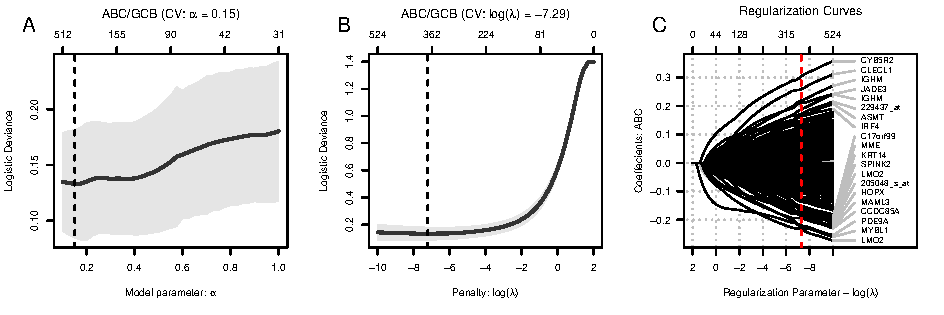
\includegraphics[width=1\textwidth]{figures/figureS1.pdf}
\end{center}
\caption{Ten fold cross validation for the parameters $\alpha$ and $\lambda$ in a logistic regression regularized by elastic net.
In panels A and B the deviance is plotted against the model parameter $\alpha$ and regularization parameter $\lambda$, respectively.
In Panel C the regularization curves are shown.
Black and grey curves represent selected and non-selected probe-sets, respectively.
Positive and negative coefficients indicate that high expression values for the associated gene are related to ABC and GCB, respectively.
The red line indicates the model chosen through $10$ fold cross validation.
The gene symbols for the $20$ probe-sets associated with the largest absolute coefficients in the chosen gene expression predictors are displayed in Panel C.}
\label{fig:crossval}
\end{figure*}

%latex.default(tableS1, file = "tables/tableS1.tex", title = "",     cgroup = names(studies.vec[-5]), rgroup = c("Wright's method",         "One-by-one", "Reference based"), size = "footnotesize",     label = "tab:confusionABCGCBHEMA", caption = caption)%
\begin{table}[!tbp]
{\footnotesize
\caption{Confusion tables for the ABC/GCB classifiers.
The columns represent cohort based normalisation using the ABC/GCB classifier
based on elastic net.
The first part of the table compares Wright's method for ABC/GCB classification
with the elastic net based.
In the second and third part one-by-one and reference based normalisation is
compared to cohort based normalisation using the ABC/GCB classifier based on
elastic net.\label{tab:confusionABCGCBHEMA}} 
\begin{center}
\begin{tabular}{lrrrcrrrcrrrcrrr}
\hline\hline
\multicolumn{1}{l}{\bfseries }&\multicolumn{3}{c}{\bfseries CHEPRETRO}&\multicolumn{1}{c}{\bfseries }&\multicolumn{3}{c}{\bfseries MDFCI}&\multicolumn{1}{c}{\bfseries }&\multicolumn{3}{c}{\bfseries IDRC}&\multicolumn{1}{c}{\bfseries }&\multicolumn{3}{c}{\bfseries LLMPP R-CHOP}\tabularnewline
\cline{2-4} \cline{6-8} \cline{10-12} \cline{14-16}
\multicolumn{1}{l}{}&\multicolumn{1}{c}{ABC}&\multicolumn{1}{c}{NC}&\multicolumn{1}{c}{GCB}&\multicolumn{1}{c}{}&\multicolumn{1}{c}{ABC}&\multicolumn{1}{c}{NC}&\multicolumn{1}{c}{GCB}&\multicolumn{1}{c}{}&\multicolumn{1}{c}{ABC}&\multicolumn{1}{c}{NC}&\multicolumn{1}{c}{GCB}&\multicolumn{1}{c}{}&\multicolumn{1}{c}{ABC}&\multicolumn{1}{c}{NC}&\multicolumn{1}{c}{GCB}\tabularnewline
\hline
{\bfseries Wright's method}&&&&&&&&&&&&&&&\tabularnewline
~~ABC&$38$&$2$&$ 0$&&$28$&$14$&$ 0$&&$174$&$23$&$  1$&&$90$&$ 3$&$  0$\tabularnewline
~~NC&$ 1$&$4$&$ 0$&&$ 1$&$11$&$ 3$&&$  6$&$26$&$ 12$&&$ 6$&$19$&$  8$\tabularnewline
~~GCB&$ 0$&$2$&$42$&&$ 0$&$ 1$&$29$&&$  5$&$31$&$189$&&$ 0$&$ 5$&$102$\tabularnewline
\hline
{\bfseries One-by-one}&&&&&&&&&&&&&&&\tabularnewline
~~ABC&$34$&$0$&$ 0$&&$24$&$ 0$&$ 0$&&$ 95$&$ 0$&$  0$&&$76$&$ 0$&$  0$\tabularnewline
~~NC&$ 5$&$2$&$ 0$&&$ 6$&$ 4$&$ 0$&&$102$&$19$&$  0$&&$20$&$ 6$&$  0$\tabularnewline
~~GCB&$ 0$&$6$&$42$&&$ 0$&$22$&$35$&&$  4$&$67$&$208$&&$ 0$&$21$&$110$\tabularnewline
\hline
{\bfseries Reference based}&&&&&&&&&&&&&&&\tabularnewline
~~ABC&$29$&$6$&$ 0$&&$16$&$ 0$&$ 0$&&$153$&$ 0$&$  0$&&$89$&$22$&$  3$\tabularnewline
~~NC&$ 0$&$1$&$ 4$&&$ 2$&$12$&$ 0$&&$ 32$&$36$&$  0$&&$ 0$&$ 0$&$ 28$\tabularnewline
~~GCB&$ 0$&$0$&$19$&&$ 0$&$ 6$&$25$&&$  0$&$42$&$202$&&$ 0$&$ 0$&$ 61$\tabularnewline
\hline
\end{tabular}\end{center}}

\end{table}

%latex.default(tableS2, file = "tables/tableS2.tex", title = "",     rgroup = flip(studies.vec)[names(subtab)], cgroup = c("One-by-one normalisation",         "Reference based"), size = "small", label = "tab:BAGShemaclass",     caption = caption)%
\begin{table}[!tbp]
{\small
\caption{Confusion tables for the BAGS classifier. One-by-one and reference
based normalisation are shown in the columns and cohort normalisation in the
rows.\label{tab:BAGShemaclass}} 
\begin{center}
\begin{tabular}{lrrrrrrcrrrrrr}
\hline\hline
\multicolumn{1}{l}{\bfseries }&\multicolumn{6}{c}{\bfseries One-by-one normalisation}&\multicolumn{1}{c}{\bfseries }&\multicolumn{6}{c}{\bfseries Reference based}\tabularnewline
\cline{2-7} \cline{9-14}
\multicolumn{1}{l}{}&\multicolumn{1}{c}{N}&\multicolumn{1}{c}{CB}&\multicolumn{1}{c}{CC}&\multicolumn{1}{c}{M}&\multicolumn{1}{c}{PB}&\multicolumn{1}{c}{UC}&\multicolumn{1}{c}{}&\multicolumn{1}{c}{N}&\multicolumn{1}{c}{CB}&\multicolumn{1}{c}{CC}&\multicolumn{1}{c}{M}&\multicolumn{1}{c}{PB}&\multicolumn{1}{c}{UC}\tabularnewline
\hline
{\bfseries CHEPRETRO}&&&&&&&&&&&&&\tabularnewline
~~Naive&$1$&$ 0$&$  0$&$0$&$ 0$&$ 1$&&$ 2$&$ 0$&$  0$&$ 0$&$ 0$&$ 0$\tabularnewline
~~Centroblast&$0$&$18$&$  0$&$0$&$ 0$&$ 0$&&$ 0$&$ 4$&$  4$&$ 0$&$ 0$&$ 1$\tabularnewline
~~Centrocyte&$0$&$10$&$ 11$&$0$&$ 5$&$ 9$&&$ 0$&$ 0$&$ 25$&$ 1$&$ 0$&$ 0$\tabularnewline
~~Memory&$0$&$ 0$&$  0$&$3$&$ 0$&$ 1$&&$ 0$&$ 0$&$  0$&$ 2$&$ 0$&$ 0$\tabularnewline
~~Plasmablast&$0$&$ 0$&$  0$&$0$&$16$&$ 0$&&$ 0$&$ 0$&$  0$&$ 0$&$ 8$&$ 3$\tabularnewline
~~Unclassified&$0$&$ 7$&$  0$&$0$&$ 4$&$ 3$&&$ 0$&$ 0$&$  2$&$ 2$&$ 0$&$ 5$\tabularnewline
\hline
{\bfseries MDFCI}&&&&&&&&&&&&&\tabularnewline
~~Naive&$1$&$ 1$&$  0$&$1$&$ 2$&$ 3$&&$ 3$&$ 0$&$  0$&$ 1$&$ 0$&$ 2$\tabularnewline
~~Centroblast&$0$&$18$&$  0$&$0$&$ 1$&$ 0$&&$ 0$&$ 9$&$  0$&$ 0$&$ 0$&$ 3$\tabularnewline
~~Centrocyte&$0$&$ 7$&$  8$&$2$&$10$&$ 6$&&$ 0$&$ 0$&$ 22$&$ 1$&$ 0$&$ 1$\tabularnewline
~~Memory&$0$&$ 0$&$  0$&$6$&$ 0$&$ 0$&&$ 0$&$ 0$&$  0$&$ 5$&$ 0$&$ 0$\tabularnewline
~~Plasmablast&$0$&$ 0$&$  0$&$0$&$11$&$ 0$&&$ 0$&$ 0$&$  0$&$ 0$&$ 7$&$ 0$\tabularnewline
~~Unclassified&$0$&$ 1$&$  0$&$1$&$ 7$&$ 5$&&$ 1$&$ 0$&$  0$&$ 2$&$ 1$&$ 3$\tabularnewline
\hline
{\bfseries IDRC}&&&&&&&&&&&&&\tabularnewline
~~Naive&$0$&$ 0$&$  3$&$0$&$ 6$&$ 4$&&$12$&$ 0$&$  0$&$ 0$&$ 1$&$ 0$\tabularnewline
~~Centroblast&$0$&$16$&$ 27$&$0$&$27$&$22$&&$ 2$&$62$&$  2$&$ 0$&$ 5$&$12$\tabularnewline
~~Centrocyte&$0$&$ 0$&$140$&$0$&$39$&$18$&&$ 1$&$ 2$&$146$&$ 7$&$ 8$&$18$\tabularnewline
~~Memory&$0$&$ 0$&$  1$&$8$&$20$&$10$&&$ 0$&$ 0$&$  0$&$35$&$ 3$&$ 1$\tabularnewline
~~Plasmablast&$0$&$ 0$&$  1$&$0$&$74$&$ 4$&&$ 0$&$ 0$&$  0$&$ 1$&$76$&$ 1$\tabularnewline
~~Unclassified&$0$&$ 0$&$ 14$&$0$&$44$&$17$&&$ 7$&$ 0$&$  0$&$ 9$&$16$&$38$\tabularnewline
\hline
{\bfseries LLMPP R-CHOP}&&&&&&&&&&&&&\tabularnewline
~~Naive&$1$&$ 2$&$  0$&$0$&$ 5$&$ 6$&&$ 8$&$ 0$&$  0$&$ 1$&$ 0$&$ 1$\tabularnewline
~~Centroblast&$0$&$32$&$  0$&$0$&$ 2$&$ 7$&&$ 0$&$37$&$  1$&$ 0$&$ 0$&$ 1$\tabularnewline
~~Centrocyte&$0$&$ 5$&$ 54$&$0$&$18$&$12$&&$ 0$&$ 1$&$ 66$&$ 1$&$ 1$&$ 4$\tabularnewline
~~Memory&$0$&$ 0$&$  0$&$5$&$13$&$ 4$&&$ 0$&$ 0$&$  0$&$22$&$ 0$&$ 0$\tabularnewline
~~Plasmablast&$0$&$ 0$&$  0$&$0$&$32$&$ 0$&&$ 0$&$ 0$&$  0$&$ 1$&$24$&$ 4$\tabularnewline
~~Unclassified&$0$&$ 2$&$  0$&$0$&$27$&$ 6$&&$ 7$&$ 1$&$  0$&$ 1$&$ 0$&$21$\tabularnewline
\hline
\end{tabular}\end{center}}

\end{table}

%latex.default(tableS3, file = "tables/tableS3.tex", title = "",     rgroup = names(subtab$onebyone), cgroup = flip(studies.vec)[names(subtab$onebyone[[1]])],     size = "small", label = "tab:confusiondrugonebyone", caption = captionS3)%
\begin{table}[!tbp]
\begin{adjustwidth}{-1in}{0in}
{\small
\caption{Confusion tables for the REGS classifiers.
One-by-one normalization are shown in the rows and cohort normalization in the
columns.\label{tab:confusiondrugonebyone}} 
\begin{center}
\begin{tabular}{lrrrcrrrcrrrcrrr}
\hline\hline
\multicolumn{1}{l}{\bfseries }&\multicolumn{3}{c}{\bfseries CHEPRETRO}&\multicolumn{1}{c}{\bfseries }&\multicolumn{3}{c}{\bfseries MDFCI}&\multicolumn{1}{c}{\bfseries }&\multicolumn{3}{c}{\bfseries IDRC}&\multicolumn{1}{c}{\bfseries }&\multicolumn{3}{c}{\bfseries LLMPP R-CHOP}\tabularnewline
\cline{2-4} \cline{6-8} \cline{10-12} \cline{14-16}
\multicolumn{1}{l}{}&\multicolumn{1}{c}{Sen}&\multicolumn{1}{c}{Int}&\multicolumn{1}{c}{Res}&\multicolumn{1}{c}{}&\multicolumn{1}{c}{Sen}&\multicolumn{1}{c}{Int}&\multicolumn{1}{c}{Res}&\multicolumn{1}{c}{}&\multicolumn{1}{c}{Sen}&\multicolumn{1}{c}{Int}&\multicolumn{1}{c}{Res}&\multicolumn{1}{c}{}&\multicolumn{1}{c}{Sen}&\multicolumn{1}{c}{Int}&\multicolumn{1}{c}{Res}\tabularnewline
\hline
{\bfseries Cyclophosphamide}&&&&&&&&&&&&&&&\tabularnewline
~~Sensitive&$40$&$ 1$&$ 0$&&$34$&$ 5$&$ 0$&&$178$&$  0$&$  0$&&$108$&$ 2$&$ 0$\tabularnewline
~~Intermediate&$ 6$&$17$&$ 0$&&$ 0$&$15$&$ 6$&&$114$&$  0$&$  0$&&$  8$&$32$&$ 1$\tabularnewline
~~Resistant&$ 0$&$ 3$&$22$&&$ 0$&$ 1$&$30$&&$203$&$  0$&$  0$&&$  0$&$15$&$67$\tabularnewline
\hline
{\bfseries Doxorubicin}&&&&&&&&&&&&&&&\tabularnewline
~~Sensitive&$30$&$ 0$&$ 0$&&$29$&$ 0$&$ 0$&&$ 25$&$ 86$&$ 39$&&$ 77$&$ 0$&$ 0$\tabularnewline
~~Intermediate&$21$&$ 6$&$ 0$&&$32$&$ 0$&$ 0$&&$  0$&$  6$&$170$&&$ 78$&$ 1$&$ 0$\tabularnewline
~~Resistant&$ 0$&$14$&$18$&&$ 6$&$12$&$12$&&$  0$&$  0$&$169$&&$ 13$&$43$&$21$\tabularnewline
\hline
{\bfseries Vincristine}&&&&&&&&&&&&&&&\tabularnewline
~~Sensitive&$36$&$ 0$&$ 0$&&$33$&$ 0$&$ 0$&&$ 42$&$ 90$&$ 33$&&$ 78$&$ 0$&$ 0$\tabularnewline
~~Intermediate&$ 7$&$ 9$&$ 0$&&$24$&$ 2$&$ 0$&&$  1$&$ 17$&$136$&&$ 59$&$15$&$ 0$\tabularnewline
~~Resistant&$ 1$&$10$&$26$&&$ 1$&$15$&$16$&&$  1$&$  3$&$172$&&$ 11$&$36$&$34$\tabularnewline
\hline
{\bfseries Combined}&&&&&&&&&&&&&&&\tabularnewline
~~Sensitive&$32$&$ 0$&$ 0$&&$33$&$ 0$&$ 0$&&$135$&$ 14$&$  1$&&$ 87$&$ 0$&$ 0$\tabularnewline
~~Intermediate&$19$&$ 9$&$ 0$&&$27$&$ 1$&$ 0$&&$ 19$&$143$&$ 21$&&$ 70$&$ 0$&$ 0$\tabularnewline
~~Resistant&$ 0$&$13$&$16$&&$ 3$&$13$&$14$&&$  0$&$ 27$&$135$&&$ 16$&$42$&$18$\tabularnewline
\hline
\end{tabular}\end{center}}
\end{adjustwidth}
\end{table}

%latex.default(tableS4, file = "tables/tableS4.tex", title = "",     rgroup = names(subtab$refbased), cgroup = flip(studies.vec)[names(subtab$refbased[[1]])],     size = "small", label = "tab:confusiondrugreference", caption = captionS4)%
\begin{table}[!tbp]
{\small
\caption{Confusion tables for the REGS classifiers.
Reference based normalisation are shown in the rows and cohort normalisation in
the columns. Note, 30 samples were used as reference data and hence not present
in this table.\label{tab:confusiondrugreference}} 
\begin{center}
\begin{tabular}{lrrrcrrrcrrrcrrr}
\hline\hline
\multicolumn{1}{l}{\bfseries }&\multicolumn{3}{c}{\bfseries CHEPRETRO}&\multicolumn{1}{c}{\bfseries }&\multicolumn{3}{c}{\bfseries MDFCI}&\multicolumn{1}{c}{\bfseries }&\multicolumn{3}{c}{\bfseries IDRC}&\multicolumn{1}{c}{\bfseries }&\multicolumn{3}{c}{\bfseries LLMPP R-CHOP}\tabularnewline
\cline{2-4} \cline{6-8} \cline{10-12} \cline{14-16}
\multicolumn{1}{l}{}&\multicolumn{1}{c}{Sen}&\multicolumn{1}{c}{Int}&\multicolumn{1}{c}{Res}&\multicolumn{1}{c}{}&\multicolumn{1}{c}{Sen}&\multicolumn{1}{c}{Int}&\multicolumn{1}{c}{Res}&\multicolumn{1}{c}{}&\multicolumn{1}{c}{Sen}&\multicolumn{1}{c}{Int}&\multicolumn{1}{c}{Res}&\multicolumn{1}{c}{}&\multicolumn{1}{c}{Sen}&\multicolumn{1}{c}{Int}&\multicolumn{1}{c}{Res}\tabularnewline
\hline
{\bfseries Cyclophosphamide}&&&&&&&&&&&&&&&\tabularnewline
~~Sensitive&$13$&$10$&$ 0$&&$26$&$ 4$&$ 0$&&$134$&$ 32$&$  0$&&$89$&$ 5$&$ 0$\tabularnewline
~~Intermediate&$ 0$&$ 7$&$10$&&$ 0$&$10$&$ 1$&&$  3$&$ 77$&$ 29$&&$ 0$&$27$&$ 9$\tabularnewline
~~Resistant&$ 0$&$ 0$&$19$&&$ 0$&$ 0$&$20$&&$  0$&$  9$&$181$&&$ 0$&$ 2$&$71$\tabularnewline
\hline
{\bfseries Doxorubicin}&&&&&&&&&&&&&&&\tabularnewline
~~Sensitive&$18$&$ 2$&$ 0$&&$19$&$ 0$&$ 0$&&$132$&$  7$&$  0$&&$50$&$15$&$ 0$\tabularnewline
~~Intermediate&$ 0$&$14$&$ 2$&&$ 0$&$21$&$ 0$&&$ 24$&$143$&$  3$&&$ 0$&$55$&$13$\tabularnewline
~~Resistant&$ 0$&$ 0$&$23$&&$ 0$&$ 3$&$18$&&$  0$&$ 16$&$140$&&$ 0$&$ 0$&$70$\tabularnewline
\hline
{\bfseries Vincristine}&&&&&&&&&&&&&&&\tabularnewline
~~Sensitive&$18$&$ 5$&$ 0$&&$16$&$ 6$&$ 0$&&$127$&$ 32$&$  0$&&$71$&$ 0$&$ 0$\tabularnewline
~~Intermediate&$ 0$&$10$&$ 1$&&$ 0$&$ 8$&$ 9$&&$ 12$&$ 83$&$ 46$&&$ 9$&$49$&$ 0$\tabularnewline
~~Resistant&$ 0$&$ 0$&$25$&&$ 0$&$ 0$&$22$&&$  1$&$ 10$&$154$&&$ 0$&$10$&$64$\tabularnewline
\hline
{\bfseries Combined}&&&&&&&&&&&&&&&\tabularnewline
~~Sensitive&$19$&$ 3$&$ 0$&&$23$&$ 1$&$ 0$&&$125$&$ 14$&$  0$&&$64$&$12$&$ 0$\tabularnewline
~~Intermediate&$ 0$&$11$&$ 5$&&$ 0$&$16$&$ 0$&&$ 12$&$148$&$ 14$&&$ 0$&$46$&$10$\tabularnewline
~~Resistant&$ 0$&$ 0$&$21$&&$ 0$&$ 0$&$21$&&$  0$&$  6$&$146$&&$ 0$&$ 0$&$71$\tabularnewline
\hline
\end{tabular}\end{center}}

\end{table}

\clearpage



\section{Graham's formula}
\label{sec:graham}
This section derives Graham's formula which, in our context, yields the posterior probability of being sensitive to the combination of two drugs, given sensitivity to the individual drugs.
For simplicity, the formula is derived for two drugs.
The formula straightforwardly generalizes to three or more drugs.

Let $C$, $H$, and $B$ be Bernoulli distributed random variables with probability parameter $1/2$, where
$C = 1$ indicates sensitivity to Cyclophosphamide $C$,
$H = 1$ indicates sensitivity to Doxorubicin $H$, and
$B = 1$ indicates sensitivity to the combination of $H$ and $C$.
Conversely, $C,H,$ and $B = 0$ indicates resistance towards $C,H,$ and $B$, respectively.
Under an assumption of conditional drug independence
\begin{align*}
  P(C=1, H=1| B=1) &= P(C=1 | B=1) P(H=1 | B=1), \text{ and } \\
  P(C=1, H=1| B=0) &= P(C=1 | B=0) P(H=1 | B=0)
\end{align*}
we have that
\begin{align*}
  &P(B=1 | H=1, C=1)
  \\&\qquad
   = \frac{P(C=1, H=1, B=1)}
          {P(C=1, H=1)}
  \\&\qquad
   = \frac{P(C=1, H=1 | B=1) P(B=1)}
          {P(C=1, H=1, B=1) + P(C=1, H=1, B=0)}
  \\&\qquad
   = \frac{P(C=1 | B=1) P(H=1 | B=1) P(B=1)}
          {P(C=1, H=1 | B=1) P(B=1) + P(H=1, C=1| B=0) P(B=0)},
\end{align*}
by the definition of conditional probabilities, the law of total probability, and the assumptions.
From the distributional assumption on $B$, $P(B=0) = P(B=1) = 1/2$, and the above then simplifies to:
\begin{equation*}
  P(B=1 | H=1, C=1)
   = \frac{P(C=1 | B=1) P(H=1 | B=1)}
          {P(C=1, H=1 | B=1) + P(H=1, C=1 | B=0)}.
\end{equation*}
For notational convenience, we abbreviate
$p_C = P(C=1 | B=1)$,
$p_H = P(H=1 | B=1)$,
$p_{CH} = P(B=1 | H=1, C=1)$.
The distributional assumptions then imply:
\begin{align*}
  p_{CH}
  &= \frac{p_C p_H}
          {p_C p_H + P(C=1 | B=0) P(H=1 | B=0)}
  \\
  &= \frac{p_C p_H}
          {p_C p_H + P(B=0 | C=1) P(B=0 | H=1)}
  \\
  &= \frac{p_C p_H}
          {p_C p_H + \bigl(1 - P(B=1 | C=1)\bigr)\bigl(1 - P(B=1 | H=1)\bigr)}
  \\
  &= \frac{p_C p_H}
          {p_C p_H + (1 - p_C)(1 - p_H)},
\end{align*}
which is the two-drug equivalent to the used formula.




\section{RMA normalization}
Recall that ordinary robust multichip average (RMA) pre-processing consists of three steps: (1) Background adjustment, (2) quantile normalization, and (3) summarization of probes to probe-sets, see e.g.\ \citep{Irizarry2003, Irizarry2003b}. For completeness we review ordinary cohort based RMA normalization.

\subsection{Backgroud correction}
In order to produce background adjusted probe intensities we will use the within array normal-exponential de-convolution scheme as implemented by the \texttt{rma.background.correct} command in the Bioconductor package \texttt{preprocessCores}, see
\citep{Irizarry2003b,Bolstad2004}.


\subsection{Quantile normalization}
Let $x_{ijk}$ be the $\log_2$-transformed and background adjusted cohort data, where $i = 1,\dots,I$ index the arrays of the cohort data, $j=1,\dots,J$  index the probe-sets, and $k=1,\dots,K_j$ index the probes nested within probe-sets.

Furthermore, let $G_i$ denote the empirical cumulative distribution function (ECDF) of the probes $\{x_{ijk}\}_{jk}$ on the $i$'th cohort array and $F$ the ECDF of the across array averaged sample quantiles $\{\bar{x}_{\cdot (jk)}\}_{ij}$, where $\{x_{i(jk)}\}_{jk}$ is the order statistic of all probes on the $i$'th cohorte array based on the lexicographic ordering of the indices $\{jk\}$. Then each data point is quantile normalized in the following way
\begin{equation*}
     \tilde{x}_{ijk} = F^{-1}(G_i(x_{ijk})),
\end{equation*}
where $F^{-1}$ is calculated as the quantiles of type 2 \citep{Hyndman1996}.
This step is performed by the \texttt{RMA\_norm} function with option \texttt{generateQuan} equal to one in the \hemaClass{} package.

\subsection{Summarisation}

For each probe-set $j$ we let $\mu_{ij}$ represent the $\log_2$-scale expression level for array $i$ and probeset $j$, $\alpha_{jk}$ the probe affinity effect, and the $\epsilon_{ijk}$'s are independent identically distributed  error terms with mean 0 and formulate the following linear additive model
\begin{equation*}
   \tilde{x}_{ijk} = \mu_{ij} + \alpha_{jk}+ \epsilon_{ijk},
\end{equation*}
where $\sum_{k=0}^{n_j} \alpha_{jk} = 0$ for all probe-sets. The parameters are estimated by median polish \citep{Holder2001}. The probe affinity estimates are denoted by $\hat{\alpha}_{jk}$.

The RMA normalized cohort data are then given by
\begin{equation*}
   \hat{x}_{ij\cdot} = \hat{\mu}_{ij},
\end{equation*}
where the dot notation indicate the mean across the index.
This step is performed by the \texttt{RMA\_sum} function in the \hemaClass{} package.




\section{One-by-one RMA normalization of user supplied data}
\subsection{Backgroud correction}

The background correction in one-by-one RMA normalization is unaltered as it is already works in an one-by-one fashion.


\subsection{Quantile normalization}

Let $x_{ijk}$ be the $\log_2$-transformed and background corrected reference data, where $i = 1,\dots,I_R$ index the arrays of the reference data, $j=1,\dots,J$  index the probe-sets, and $k=1,\dots,K_j$ index the probes. Assume $x_{ijk}$ has been RMA normalized as described above. Similarly,  let $y_{ijk}$ be the log2-transformed and background corrected user supplied data, where $i = 1,\dots,I_U$ index the arrays of the user supplied data, $j=1,\dots,J$  index the probe-sets, and $k=1,\dots,K_j$ index the probes.

Furthermore, let $H_i$ denote the ECDF of the user supplied data $\{y_{ijk}\}_{jk}$, respectively.

As quantile normalizer the ECDF of the background corrected reference data is used in place of the ususally applied ECDF of the mean of the sample quantiles
\begin{equation*}
   \tilde{y}_{ijk} = F^{-1}(H_i(y_{ijk})).
\end{equation*}
This step is performed by the \texttt{RMA\_norm} function with options \texttt{generateQuan} equal to zero and \texttt{quantile} equal to the quantiles of the reference data in the \hemaClass{} package.


\subsection{Summarization}

To mimic the RMA summarization the probe effects estimated by median polish on the reference data is subtracted all probes of the user data
\begin{equation*}
   \hat{y}_{ijk} = \tilde{y}_{ijk} - \hat{\alpha}_{jk},
\end{equation*}
in place of the usual estimated probe effects from the cohort.
The pre-processed expression value for each probe-set is then estimated as the median of the associated probes.
\begin{equation*}
   \hat{y}_{ij\cdot} = \median_{k \in \{1,\dots,n_j \}} \{ \hat{y}_{ijk} \}.
\end{equation*}


\section{Classification}
To ensure identical classification probabilities whether data is supplied as a cohort or one-by-one, we finally subtract the median of each probe-set in the reference from the corresponding probe-set and scale by the standard deviation of each probe-set in the reference data
\begin{equation*}
  (\hat{y}_{ij\cdot} - \hat{x}_{\cdot j\cdot})/s_{\cdot j\cdot},
\end{equation*}
where
$\hat{x}_{\cdot j\cdot} = \median_{i \in \{1,\dots,I_R \}} \{\hat{x}_{ij\cdot}\}$ and $s_{\cdot j\cdot} = \std_{i \in \{1,\dots,I_R\}} \{\hat{x}_{ij\cdot}\}$.


% \end{document}

% \cleardoublepage
% \listoftodos









\end{document}







